\documentclass[preprint,12pt]{elsarticle}

%% Use the option review to obtain double line spacing
%% \documentclass[preprint,review,12pt]{elsarticle}

%% Use the options 1p,twocolumn; 3p; 3p,twocolumn; 5p; or 5p,twocolumn
%% for a journal layout:
%% \documentclass[final,1p,times]{elsarticle}
%% \documentclass[final,1p,times,twocolumn]{elsarticle}
%% \documentclass[final,3p,times]{elsarticle}
%% \documentclass[final,3p,times,twocolumn]{elsarticle}
%% \documentclass[final,5p,times]{elsarticle}
%% \documentclass[final,5p,times,twocolumn]{elsarticle}

%% The graphicx package provides the includegraphics command.
\usepackage{graphicx}
%% The amssymb package provides various useful mathematical symbols
\usepackage{amssymb}
%% The amsthm package provides extended theorem environments
%% \usepackage{amsthm}

%% The lineno packages adds line numbers. Start line numbering with
%% \begin{linenumbers}, end it with \end{linenumbers}. Or switch it on
%% for the whole article with \linenumbers after \end{frontmatter}.
% \usepackage{lineno}

\usepackage{mathtools}
\usepackage{subcaption}

%% add pseudo codes
\usepackage{algorithm}
\usepackage{algorithmicx}
\usepackage{algpseudocode}

\floatname{algorithm}{Algorithm}
\renewcommand{\algorithmicrequire}{\textbf{INPUT:}}
\renewcommand{\algorithmicensure}{\textbf{OUTPUT:}}

%% add python codes
\usepackage{listings}
\usepackage{color}

\definecolor{dkgreen}{rgb}{0,0.6,0}
\definecolor{gray}{rgb}{0.5,0.5,0.5}
\definecolor{mauve}{rgb}{0.58,0,0.82}

\lstset{frame=tb,
  language=Python,
  aboveskip=3mm,
  belowskip=3mm,
  showstringspaces=false,
  columns=flexible,
  basicstyle={\small\ttfamily},
  numbers=none,
  numberstyle=\tiny\color{gray},
  keywordstyle=\color{blue},
  commentstyle=\color{dkgreen},
  stringstyle=\color{mauve},
  breaklines=true,
  breakatwhitespace=true,
  tabsize=3
}

%% natbib.sty is loaded by default. However, natbib options can be
%% provided with \biboptions{...} command. Following options are
%% valid:

%%   round  -  round parentheses are used (default)
%%   square -  square brackets are used   [option]
%%   curly  -  curly braces are used      {option}
%%   angle  -  angle brackets are used    <option>
%%   semicolon  -  multiple citations separated by semi-colon
%%   colon  - same as semicolon, an earlier confusion
%%   comma  -  separated by comma
%%   numbers-  selects numerical citations
%%   super  -  numerical citations as superscripts
%%   sort   -  sorts multiple citations according to order in ref. list
%%   sort&compress   -  like sort, but also compresses numerical citations
%%   compress - compresses without sorting
%%
%% \biboptions{comma,round}

% \biboptions{}

\journal{}

\begin{document}

\begin{frontmatter}

%% Title, authors and addresses

\title{Solutions of Equations in One Variable}

%% use the tnoteref command within \title for footnotes;
%% use the tnotetext command for the associated footnote;
%% use the fnref command within \author or \address for footnotes;
%% use the fntext command for the associated footnote;
%% use the corref command within \author for corresponding author footnotes;
%% use the cortext command for the associated footnote;
%% use the ead command for the email address,
%% and the form \ead[url] for the home page:
%%
%% \title{Title\tnoteref{label1}}
%% \tnotetext[label1]{}
%% \author{Name\corref{cor1}\fnref{label2}}
%% \ead{email address}
%% \ead[url]{home page}
%% \fntext[label2]{}
%% \cortext[cor1]{}
%% \address{Address\fnref{label3}}
%% \fntext[label3]{}


%% use optional labels to link authors explicitly to addresses:
%% \author[label1,label2]{<author name>}
%% \address[label1]{<address>}
%% \address[label2]{<address>}

\author{ChaosWSF}

\address{No.0, University}

\begin{abstract}
%% Text of abstract
The purpose of this report is to obtain the approximate solutions to the equation in single variable. Taken the accuracy and convergence speed into consideration, there are three methods mentioned in the report, namely Newton's method, Horner's method and M\"uller's method. Though Horner's method has become a tool to improve the accuracy of polynomial multiplication, the concept of deflation is still essential for the search of all zeros of the polynomial. Then several experiments have been done to verify the effectiveness of those root-finding methods. Based on results of such experiments, it can be observed that those methods are effective and fast.
\end{abstract}

\begin{keyword}
Newton's method \sep Horner's method \sep M{\"u}ller's method
%% keywords here, in the form: keyword \sep keyword

%% MSC codes here, in the form: \MSC code \sep code
%% or \MSC[2008] code \sep code (2000 is the default)

\end{keyword}

\end{frontmatter}

%%
%% Start line numbering here if you want
%%
% \linenumbers

%% main text
\section{Introduction}
\label{S:1}

In mathematics and computing, a root-finding algorithm is an algorithm for finding roots of continuous functions. A root of a function $f$ is a number $x$ such that $f(x)=0$. As, the roots of a function cannot be computed exactly, nor expressed in closed form, root-finding algorithms provide approximations to roots, expressed either as floating point numbers or as small isolating intervals, or disks for complex roots.

Solving an equation $f(x)=g(x)$ is the same as finding the roots of the function $h(x)=f(x)-g(x)$. Thus root-finding algorithms allow solving any equation defined by continuous functions. However, most root-finding algorithms do not guarantee that they will find all the roots; in particular, if such an algorithm does not find any root, that does not mean that no root exists.

Most numerical root-finding methods use iteration, producing a sequence of numbers that hopefully converge towards the root as a limit. They require one or more initial guesses of the root as starting values, then each iteration of the algorithm produces a successively more accurate approximation to the root. Since the iteration must be stopped at some point these methods produce an approximation to the root, not an exact solution. Many methods compute subsequent values by evaluating an auxiliary function on the preceding values. The limit is thus a fixed point of the auxiliary function, which is chosen for having the roots of the original equation as fixed points, and for converging rapidly to these fixed points.

The behaviour of general root-finding algorithms is studied in numerical analysis. However, for polynomials, root-finding study belongs generally to computer algebra, since algebraic properties of polynomials are fundamental for the most efficient algorithms. The efficiency of an algorithm may depend dramatically on the characteristics of the given functions. For example, many algorithms use the derivative of the input function, while others work on every continuous function. In general, numerical algorithms are not guaranteed to find all the roots of a function, so failing to find a root does not prove that there is no root. However, for polynomials, there are specific algorithms that use algebraic properties for certifying that no root is missed, and locating the roots in separate intervals (or disks for complex roots) that are small enough to ensure the convergence of numerical methods (typically Newton's method) to the unique root so located.

The name "Newton's method" is derived from Isaac Newton's description of a special case of the method. However, his method differs substantially from the modern method given above: Newton applies the method only to polynomials. He does not compute the successive approximations $x_n$, but computes a sequence of polynomials, and only at the end arrives at an approximation for the root $x$. Finally, Newton views the method as purely algebraic and makes no mention of the connection with calculus. Newton may have derived his method from a similar but less precise method by Vieta. The essence of Vieta's method can be found in the work of the Persian mathematician, while his successor used a form of Newton's method to solve $x^P-N=0$ to find roots of $N$. A special case of Newton's method for calculating square roots was known much earlier and is often called the Babylonian method.

Newton's method was first published in 1685 in \textit{A Treatise of Algebra both Historical and Practical} by John Wallis. In 1690, Joseph Raphson published a simplified description in \textit{Analysis aequationum universalis}. Raphson again viewed Newton's method purely as an algebraic method and restricted its use to polynomials, but he describes the method in terms of the successive approximations $x_n$ instead of the more complicated sequence of polynomials used by Newton. Finally, in 1740, Thomas Simpson described Newton's method as an iterative method for solving general nonlinear equations using calculus, essentially giving the description above. In the same publication, Simpson also gives the generalization to systems of two equations and notes that Newton's method can be used for solving optimization problems by setting the gradient to zero.

Arthur Cayley in 1879 in \textit{The Newton-Fourier imaginary problem} was the first to notice the difficulties in generalizing Newton's method to complex roots of polynomials with degree greater than 2 and complex initial values. This opened the way to the study of the theory of iterations of rational functions.

Except Newton's method, there still have been lots of root-finding algorithm nowadays. In this report, several popular and essential methods would be introduced and verified by experiment. Those methods are designed for general continuous functions or the polynomials. With good application of them, the accuracy and convergence speed of root-finding can be improved significantly.

\section{Methodologies}
\label{S:2}

There are several methods to approximate the solutions of an equation in one variable, which are introduced in \cite{burden:2001qr}. In this section, three methods are shown, due to their popularity and accuracy, which are also listed below.

\begin{itemize}
\item Newton's method
\item Horner's method
\item M\"uller's method
\end{itemize}

% \begin{enumerate}
% \item Numbered list item one
% \item Numbered list item two
% \end{enumerate}

All these methods can be used to obtain the zeros of polynomials through some skills, such as varying the initial values. And Newton's method and M\"uller's method can be applied to more general functions which have some properties (Read details in \cite{burden:2001qr}). Further, the M\"uller's method is unique among three methods because it can get the complex zeros as well.

\subsection{Introduction to Newton's Method}
\label{SS:2.1}

Newton's method is the most powerful and well-known numerical methods for solving a root-finding problem. The introduction of Newton's method below is based on Taylor polynomials.

Suppose that $f\in C^2[a,b]$. Let $\bar{x}\in[a,b]$ be an approximation to $p$ such that $f^{'}(\bar{x})\neq0$ and $|p-\bar{x}|$ is "small". Consider the first Taylor polynomial for $f(x)$ expanded about $\bar{x}$,

\begin{equation}
\label{eq:intro_newton_1}
    f(x)=f(\bar{x})+(x-\bar{x})f^{'}(\bar{x})+\frac{(x-\bar{x})^2}{2}f^{''}(\xi(x)),
\end{equation}

where $\xi(x)$ lies between $x$ and $\bar{x}$. Since $f(p)=0$, Eq. (\ref{eq:intro_newton_1}) with $x=p$ gives 

\begin{equation}
    0=f(\bar{x})+(p-\bar{x})f^{'}(\bar{x})+\frac{(p-\bar{x})^2}{2}f^{''}(\xi(p)),
\end{equation}

Newton's method is derived by assuming that since $|p-\bar{x}|$ is small, the term involving $(p-\bar{x})^2$ is much smaller, so

\begin{equation}
    0\approx f(\bar{x})+(p-\bar{x})f^{'}(\bar{x}).
\end{equation}

Solving for $p$ gives 

\begin{equation}
    p\approx \bar{x}-\frac{f(\bar{x})}{f^{'}(\bar{x})}
\end{equation}

This sets the stage for Newton's method, which starts with an initial approximation $p_0$ and generates the sequence $\{p_n\}_{n=0}^{\infty}$, by

\begin{equation}
    p_n=p_{n-1}-\frac{f(p_{n-1})}{f^{'}(p_{n-1})},\quad \forall n\geq 1
\end{equation}

In addition, the pseudo codes of Newton's method are illustrated in Algorithm \ref{algo:newton}.

\begin{algorithm}
    \caption{Newton's}
    \label{algo:newton}
    \begin{algorithmic}[1]
    \Require initial value $p_0$, tolerance $TOL$, maximum iterations $N_0$.
    \Ensure approximate solution $p$ or failure message.
    \State $i\gets 1$
    \While {$i\leq N_0$}
        \State $p\gets p_0-\frac{f(p_0)}{f^{'}(p_0)}$
        \If {$|f(p)|<TOL$}
            \State \Return $p$
        \EndIf
        \State $i\gets i+1$
        \State $p_0\gets p$
    \EndWhile
    \If {$i>N_0$}
        \State \Return "Failure"
    \EndIf
    \end{algorithmic}
\end{algorithm}

\subsection{Introduction to Horner's Method}
\label{SS:2.2}

The Horner's method is widely used and has been a standard method for hand calculation. It gives a convenient way for using the Newton's method for polynomials. It relies on the algorithm for polynomial evaluation now named after Horner. After the introduction of computers this root-finding method went out of use and as a result the term Horner's method has become understood to mean just the polynomial evaluation algorithm.

In mathematics, the term Horner's method refers to a polynomial evaluation method named after William George Horner expressed by

\begin{equation}
    \begin{split}
        p(x) &= a_0+a_1 x+a_2x^2+ a_3x^3+\dots+a_{n}x^n\\
        &= a_0+x(a_1+x(a_2+x(a_3+\dots+x(a_{n-1}+{x}a_n))\dots))).
    \end{split}
\end{equation}

This allows evaluation of a polynomial of degree $n$ with only $n$ multiplications and $n$ additions. The algorithm is described below. Given the polynomial

\begin{equation}
    p(x)=\sum_{i=0}^n{a_i x^i}=a_0+a_1 x+a_2x^2+ a_3x^3+\dots+a_{n}x^n,
\end{equation}

where $a_0,\dots,a_n$ are constant coefficients, we wish to evaluate the polynomial at a specific value of $x$ that we'll call $x_0$.

To accomplish this, we define a new sequence of constants as follows:

\begin{equation}
    \begin{split}
        b_n &:= a_n\\
        b_{n-1} &:= a_{n-1}+b_{n}x_0\\
        b_{n-2} &:= a_{n-2}+b_{n-1}x_0\\
        & \vdotswithin{:=} \\
        b_0 &:= a_0+b_1 x_0.
    \end{split}
\end{equation}

Then $b_0$ is the value of $p(x_0)$.

To see why this works, note that the polynomial can be written in the form

\begin{equation}
    p(x)=a_0+x(a_1+x(a_2+x(a_3+\dots+x(a_{n-1}+{x}a_n))\dots))).
\end{equation}

Thus, by iteratively substituting the $b_i$ into the expression, 
 
\begin{equation}
    \begin{split}
        p(x)&=a_0+x_0(a_1+x_0(a_2+\dots+x_0(a_{n-1}+b_n{x_0})\dots))\\
        &=a_0+x_0(a_1+x_0(a_2+\dots+x_0{b_{n-1}}))\\
        & \vdotswithin{=} \\
        &=a_0+x_0 b_1\\
        &=b_0.
    \end{split}
\end{equation}

The pseudo codes of Horner's method are illustrated in Algorithm \ref{algo:horner}.

\begin{algorithm}
    \caption{Horner's}
    \label{algo:horner}
    \begin{algorithmic}[1]
    \Require degree $n$; coefficients $a_0, a_1,\dots,a_n;x_0$.
    \Ensure $y=P(x_0);z=P^{'}(x_0).$
    \State $y\gets a_n$
    \State $z\gets a_n$
    \For {$j=n-1,n-2,\dots,1$}
        \State $y\gets x_0 y+a_j$
        \State $z\gets x_0 z+y$
    \EndFor
    \State $y\gets x_0 y+a_0$
    \State \Return $(y,z)$
    \end{algorithmic}
\end{algorithm}

In addition, all real zeros can be found through specific technique called deflation. If the $N$th iterate, $x_N$, in Newton's method is an approximate zero for $P$, then

\begin{equation}
    P(x)=(x-x_N)Q(x)+b_0=(x-x_N)Q(x)+P(x_N)\approx(x-x_N)Q(x),
\end{equation}

so $x-x_N$ is an approximate factor of $P(x)$. Letting $\hat{x_1}=x_N$ be the approximate zero of $P$ and $Q_1(x)\equiv Q(x)$ be the approximate factor gives

\begin{equation}
    P(x)\approx(x-\hat{x_1})Q_1(x).
\end{equation}

By applying Newton's method to $Q_1(x)$, a second approximate zero of $P$. If $P(x)$ is an $n$th-degree polynomial with $n$ real zeros, this procedure applied repeatedly will eventually result in $(n-2)$ approximate zeros of $P$ and an approximate quadratic factor $Q_{n-2}(x)$. At this stage, $Q_{n-2}(x)=0$ can be solved by the quadratic formula to find the last two approximate zeros of $P$.

\subsection{Introdcution to M\"uller's Method}
\label{SS:2.3}

M\"uller's method is similar to the Secant method. But whereas the Secant method uses a line through two points on the curve to approximate the root, M\"uller's method uses a parabola through three points on the curve for the approximation.

The Secant method begins with two initial approximations $p_0$ and $p_1$ and determines the next approximation $p_2$ as the intersection of the x-axis with the line through $(p_0,f(p_0))$ and $(p_1,f(p_1))$. (See Figure \ref{fig:muller1}.) M\"uller's method uses three initial approximations, $p_0$, $p_1$, and $p_2$, and determines the next approximation $p_3$ by considering the intersection of the x-axis with the parabola through $(p_0,f(p_0))$, $(p_1,f(p_1))$, and $(p_2,f(p_2))$. (See Figure \ref{fig:muller2}.)

\begin{figure}
\centering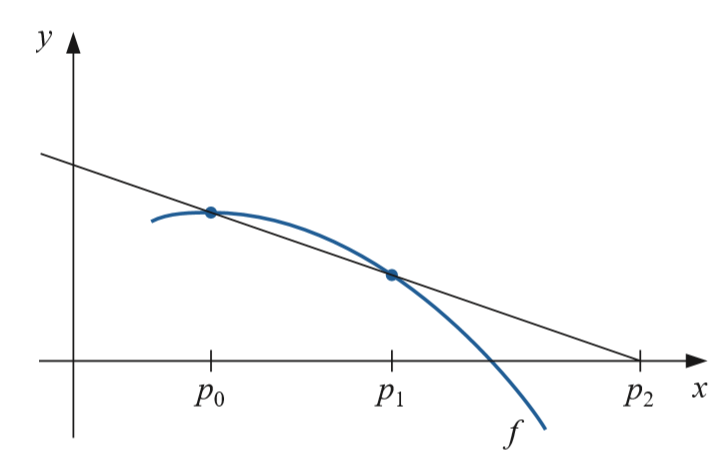
\includegraphics[width=0.4\linewidth]{muller2.png}
\caption{Secant method}
\label{fig:muller1}
\end{figure}

\begin{figure}
\centering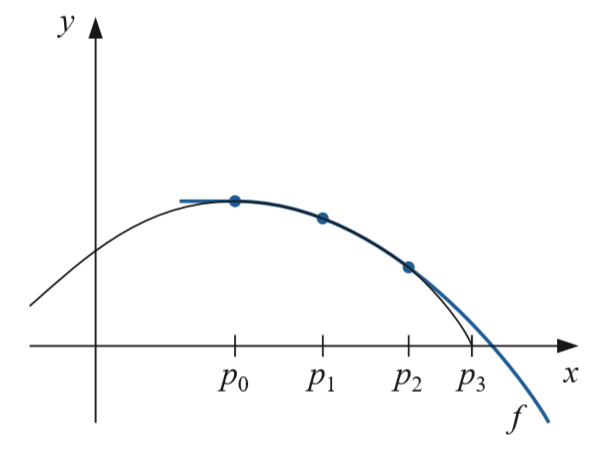
\includegraphics[width=0.4\linewidth]{muller1.png}
\caption{M\"uller's method}
\label{fig:muller2}
\end{figure}

The derivation of M\"uller's method begins by considering the quadratic polynomial 

\begin{equation}
    P(x)=a(x-p_2)^2+b(x-p_2)+c
\end{equation}

that passes through $(p_0,f(p_0))$, $(p_1,f(p_1))$, and $(p_2,f(p_2))$. The constants $a$, $b$, and $c$ can be determined from the conditions 

\begin{equation}
    f(p_0)=a(p_{0}-p_2)^2+b(p_{0}-p_2)+c,
\end{equation}
\begin{equation}
    f(p_1)=a(p_{1}-p_2)^2+b(p_{1}-p_2)+c,
\end{equation}

and

\begin{equation}
    f(p_2)=a \cdot 0^2+b\cdot 0+c=c
\end{equation}

to be

\begin{equation}
\label{eq:muller_c}
    c=f(p_2),
\end{equation}
\begin{equation}
\label{eq:muller_b}
    b=\frac{(p_{0}-p_2)^2[f(p_1)-f(p_2)]-(p_{1}-p_2)^2[f(p_0)-f(p_2)]}{(p_{0}-p_2)(p_{1}-p_2)(p_{0}-p_1)},
\end{equation}

and

\begin{equation}
\label{eq:muller_a}
    a=\frac{(p_{1}-p_2)[f(p_0)-f(p_2)]-(p_{0}-p_2)[f(p_1)-f(p_2)]}{(p_{0}-p_2)(p_{1}-p_2)(p_{0}-p_1)}.
\end{equation}

To determine $p_3$, a zero of $P$, we apply the quadratic formula to $P(x)=0$. However, because of round-off error problems caused by the subtraction of nearly equal numbers, some skills has been used here:

\begin{equation}
    p_{3}-p_2=\frac{-2c}{b\pm\sqrt{b^{2}-4ac}}.
\end{equation}

This formula gives two possibilities for $p_3$, depending on the sign preceding the radical term. In M\"uller's method, the sign is chosen to agree with the sign of $b$. Chosen in this manner, the denominator will be the largest in magnitude and will result in $p_3$ being selected as the closest zero of $P$ to $p_2$. Thus 

\begin{equation}
    p_{3}=p_{2}-\frac{2c}{b+\mathrm{sgn}(b)\sqrt{b^{2}-4ac}},
\end{equation}

where $a$, $b$, and $c$ are given in Eq. (\ref{eq:muller_c}), (\ref{eq:muller_b}), (\ref{eq:muller_a}).
Once $p_3$ is determined, the procedure is reinitialized using $p_1$, $p_2$, and $p_3$ in place of $p_0$, $p_1$, and $p_2$ to determine the next approximation, $p_4$. The method continues until a satisfactory conclusion is obtained. At each step, the method involves the radical $\sqrt{b^{2}-4ac}$, so the method gives approximate complex roots when $b^{2}-4ac<0$. The pseudo codes of M\"uller's method are illustrated in Algorithm \ref{algo:muller}.

\begin{algorithm}
    \caption{M\"uller's}
    \label{algo:muller}
    \begin{algorithmic}[1]
    \Require $p_0,p_1,p_2$; tolerance $TOL$; maximum iterations $N_0$.
    \Ensure approximate solution $p$ or failure message.
    \State $h_1\gets p_1 - p_0$
    \State $h_2\gets p_2 - p_1$
    \State $\delta_1\gets \frac{f(p_1)-f(p_0)}{h_1}$
    \State $\delta_1\gets \frac{f(p_2)-f(p_1)}{h_2}$
    \State $d\gets \frac{\delta_2 - \delta_1}{h_2 + h_1}$
    \State $i\gets 3$
    \While{$i\leq N_0$}
        \State $b\gets\delta_{2}+h_{2}d$
        \State $D\gets (b^{2}-4f(p_2)d)^{\frac{1}{2}}$
        \Comment  May require complex arithmetic.
        \If{$|b-D|<|b+D|$}
            \State $E\gets b+D$
        \Else
            \State $E\gets b-D$
        \EndIf
        \State $h\gets\frac{-2f(p_2)}{E}$
        \State $p\gets p_{2}+h$
        \If {$|h|<TOL$}
            \State \Return $p$
        \EndIf
        \State $p_0=p_1$
        \State $p_1=p_2$
        \State $p_2=p$
        \State $h_1\gets p_1 - p_0$
        \State $h_2\gets p_2 - p_1$
        \State $\delta_1\gets \frac{f(p_1)-f(p_0)}{h_1}$
        \State $\delta_1\gets \frac{f(p_2)-f(p_1)}{h_2}$
        \State $d\gets \frac{\delta_2 - \delta_1}{h_2 + h_1}$
        \State $i\gets i+1$
    \EndWhile
    \If {$i>N_0$}
        \State \Return "Failure"
    \EndIf
    \end{algorithmic}
\end{algorithm}

\section{Experiments}
\label{S:3}

In this section, several experiments are used to verify three methods which are introduced in the above section. The solving programs are written in Python and the following codes are run at first to import some useful packages.

\begin{lstlisting}
import numpy as np
\end{lstlisting}

\subsection{Newton's Method}

As is mentioned in Section \ref{SS:2.1}, the solution of an equation can be obtained by Newton's method. To verify the effectiveness of Newton's method, an equation is designed. Exactly, Newton's method is used to get the solution of Eq. (\ref{eq:newton1}) in a given interval with accuracy of $10^{-5}$.

\begin{equation}
\label{eq:newton1}
    \mathrm{e}^x + 2^{-x} + 2\cos x - 6 = 0, \quad1\leq x\leq 2
\end{equation}

To approach this problem, define $f(x)=\mathrm{e}^x + 2^{-x} + 2\cos x - 6$ and get the derivative $f^{'}(x)=\mathrm{e}^x-2^{-x}\log{2}-2\sin x $ through manual calculation. The sequence is generated by 

\begin{equation}
    p_n=p_{n-1} - \frac{\mathrm{e}^p + 2^{-p} + 2\cos{p} - 6}{\mathrm{e}^p-2^{-p}\log{2}-2\sin{p}},\quad \forall\,n\geq 1
\end{equation}

Set the initial point as $p_0=1.5$. Then running the program below, the absolute error of solution meets the requirement at the fourth iteration. 

\begin{lstlisting}
def f(x):
    return np.exp(x) + 2 ** (-x) + 2 * np.cos(x) - 6

def fprime(x):
    return np.exp(x) - np.log(2) * 2 ** (-x) - 2 * np.sin(x)

p0 = 1.5

tol = 1e-5
N = 100 # N_min = 5
p = p0
i = 1

while (i <= N) & (abs(f(p)) >= tol):
    p = p - f(p) / fprime(p)
    i = i + 1

if i > N:
    print('the root is not found')
else:
    print('the root is {0} in {1} iter'.format(p, i-1))
\end{lstlisting}

The detail of approximation process is shown in Table \ref{tab:newton}.

\begin{table}[h]
\centering
\begin{tabular}{l l l}
\hline
\textbf{$n$} & \textbf{$p_n$} & \textbf{$f(p_n)$}\\
\hline
0 & 1.5 & -1.023283135733256 \\
1 & 1.9564897211242105 & 0.5797013732749239 \\
2 & 1.8415330610420606 & 0.050340951614865403 \\
3 & 1.8295060132036511 & 0.000502121322591087 \\
4 & 1.829383614494166 & 5.151613891030138e-08 \\
5 & 1.829383601933849 & 8.881784197001252e-16 \\
6 & 1.8293836019338487 & 0.0 \\
\hline
\end{tabular}
\caption{Approximation process of Newton's method}
\label{tab:newton}
\end{table}

\subsection{Horner's Method}

As is mentioned in Section \ref{SS:2.2}, the real zeros of a polynomial can be obtained by the combination of Horner's and Newton's method. To verify the effectiveness of such combination, Eq. (\ref{eq:Horner}) is designed and the goal is to find all real zeros of it within $10^{-4}$. For the convenience of verification, the right zeros are also shown below.

\begin{equation}
\begin{split}
    P(x)&=x^4-3x^3-0.13x^2+2.37x+0.4536\\
    &=(x-1.2)(x-2.7)(x+0.2)(x+0.7)
\end{split}
\label{eq:Horner}
\end{equation}

Set the initial point as $x_0=5$ and the maximum iteration as $N=10$, which are got by trial and error. 

\begin{lstlisting}
def polynomial(x, coeff):
    y = 0
    deg = len(coeff) - 1
    for c in range(deg+1):
        y += coeff[c] * x ** (deg - c)
    return y

tol = 1e-4
N = 10
P0_coeff = [1, -3, -.13, 2.37, 0.4536]
x0 = 5

P_coeff = P0_coeff
for de in range(1, len(P0_coeff)):
    x = x0
    k = 1
    while (k <= N) & (abs(polynomial(x, P_coeff)) >= tol):
        Q_coeff = [P_coeff[0]]

        for i in range(1, len(P_coeff)):
            Q_coeff.append(P_coeff[i] + x * Q_coeff[i-1])

        b0 = Q_coeff[-1]
        Q_coeff = Q_coeff[:-1]
        Q_x = Q_coeff[0]

        for j in range(1, len(Q_coeff)):
            Q_x = Q_coeff[j] + Q_x * x

        x = x - b0 / Q_x
        k = k + 1

    if k > N:
        print('in the %dth round, the real root is not found' % de)
        break
    else:
        print('the real root is %f' % x)
        P_coeff = Q_coeff
\end{lstlisting}

Then running the program above, four real zeros are obtained, which are shown below.

$$
x_1=2.70000, \,x_2=1.19983, \,x_3=-0.20380, \,x_4=-0.69866
$$

\begin{figure}
\centering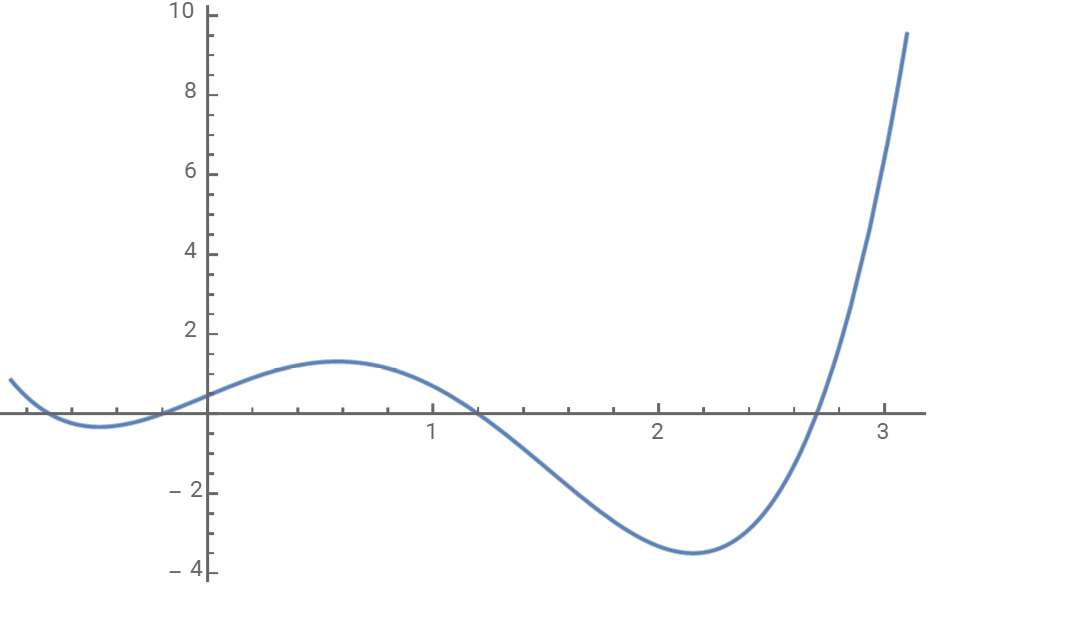
\includegraphics[width=0.8\linewidth]{Fig_poly_1.png}
\caption{Image of Eq. \ref{eq:Horner}}
\label{fig:poly1}
\end{figure}

\subsection{M\"uller's Method}

As is mentioned in Section \ref{SS:2.3}, all zeros of a polynomial can be obtained by M\"uller's method, including real and complex solutions. To verify its effectiveness, Eq. (\ref{eq:muller1}) is designed and the goal is to find all zeros of it within $10^{-4}$.

\begin{equation}
    f(x)=x^5-x^4+2x^3-3x^2+x-4
\label{eq:muller1}
\end{equation}

Unlike the experiment of Horner's method, several different initial values have to be used to get all the zeros of Eq. (\ref{eq:muller1}). 

\begin{lstlisting}
def f(x):
    return x**5 - x**4 + 2*x**3 - 3*x**2 + x - 4

tol = 1e-4
N = 20

x0 = 0.5
x1 = 1.5
x2 = 0

h1 = x1 - x0
h2 = x2 - x1
delta1 = (f(x1) - f(x0)) / h1
delta2 = (f(x2) - f(x1)) / h2
d = (delta2 - delta1) / (h2 + h1)
i = 3

while i<= N:
    b = delta2 + h2 * d
    D = np.sqrt(b**2 - 4*f(x2)*d + 0j)
    if np.abs(b+D) < np.abs(b-D):
        E = b - D
    else:
        E = b + D
    h = -2 * f(x2) / E
    p = x2 + h
    if np.abs(h) < tol:
        break
    else:
        x0 = x1
        x1 = x2
        x2 = p
        h1 = x1 - x0
        h2 = x2 - x1
        delta1 = (f(x1) - f(x0)) / h1
        delta2 = (f(x2) - f(x1)) / h2
        d = (delta2 - delta1) / (h2 + h1)
        i = i + 1

if i > N:
    print('the root is not found')
else:
#     print('the root is', p)
    print('the root is {0} in {1} iter'.format(p, i-1))
\end{lstlisting}

Running the program above, three zeros are obtained. The details are shown in the Table \ref{tab:muller}. Only three zeros are obtained by program because other two complex zeros are just conjugate to two known solutions. Thus, all zeros are listed in Table \ref{tab:muller0}.

\begin{table}[h]
\centering
\begin{tabular}{l|l}
\hline
root1 & 1.498189984970468\\
root2 & -0.5136343227538117-1.0915621843348469i\\
root3 & -0.5136343227538117+1.0915621843348469i\\
root4 & 0.26453934038943494-1.32837491492632i\\
root5 & 0.26453934038943494+1.32837491492632i\\
\hline
\end{tabular}
\caption{Zeros of Eq.\ref{eq:muller1}}
\label{tab:muller0}
\end{table}

\begin{table}[p]
    \begin{subtable}[h]{1\textwidth}
        \centering
        \begin{tabular}{l l l}
        \hline
        \textbf{$i$} & \textbf{$x_i$} & \textbf{$f(x_i)$}\\
        \hline
        3 & 1.4987641499 & 0.0098944025 \\
        4 & 1.4981893180 & -1.14795426e-05 \\
        5 & 1.4981899850 & 4.2212207e-09 \\
        6 & 1.4981899848 & 1.7763568e-15 \\
        \hline
       \end{tabular}
       \caption{$x_0=0.5,\quad x_1=1.5,\quad x_2=2$}
    \end{subtable}
    \begin{subtable}[h]{1\textwidth}
        \centering
        \begin{tabular}{l l l}
        \hline
        \textbf{$i$} & \textbf{$x_i$} & \textbf{$f(x_i)$}\\
        \hline
        3 & -0.9726770457 & -11.4172355652 \\
        4 & 1.2759007672 & -2.7225581194 \\
        5 & 0.8078752170-0.8397001337i & -4.9254634275+2.6424742169i \\
        6 & -0.3832437349-1.4452435867i & -3.6035639304+2.2701000647i \\
        7 & -0.8838301304-2.2081360516i & -41.5923605633+54.1014109354i \\
        8 & -0.3920837811-1.3448679016i & -2.2517375903+1.7872907667i \\
        9 & -0.5204394313-1.2185357102i & -0.0710979435+1.4613964953i \\
        10 & -0.5376338270-1.1410799101i & 0.2911392891+0.5397771931i \\
        11 & -0.5163812421-1.0933102388i & 0.0303434463+0.0149723139i \\
        12 & -0.5136541938-1.0915290400i & 0.0001665642-0.0003627671i \\
        13 & -0.5136343228-1.0915621843i & -9.68367937e-08+6.45063298e-08i \\
        \hline
        \end{tabular}
        \caption{$x_0=0.5,\quad x_1=1.5,\quad x_2=0$}
     \end{subtable}
     \begin{subtable}[h]{1\textwidth}
        \centering
        \begin{tabular}{l l l}
        \hline
        \textbf{$i$} & \textbf{$x_i$} & \textbf{$f(x_i)$}\\
        \hline
        3 & -0.0534781190 & -4.0623723482 \\
        4 & -0.3171415430 & -4.6959975410 \\
        5 & 0.1227895193-1.0052713356i & -1.9532986184+0.3100729674i \\
        6 & -0.0248376068-1.3186650197i &  -1.9434483806-0.6794351214i \\
        7 & 0.5358478580-1.3388275737i & 1.2837856394+3.1761120076i \\
        8 & 0.2449841391-1.3650708039i & 0.1208648845-0.4129976024i \\
        9 & 0.2702481150-1.3274984301i & 0.0312067152+0.0485842208i \\
        10 & 0.2644472564-1.3284348337i & -0.0001700517-0.0010807801i \\
        11 & 0.2645393611-1.3283748769i & -1.43693546e-07+4.06340165e-07i \\
        \hline
        \end{tabular}
        \caption{$x_0=1,\quad x_1=4,\quad x_2=0$}
     \end{subtable}
     \caption{M\"uller's method}
     \label{tab:muller}
\end{table}

Through the former example, it can be observed that M\"uller's method is powerful to solve the polynomial equation. Then a transcendental equation, Eq. (\ref{eq:muller2}), is solved by M\"uller's method to get a complex zero within $10^{-5}$.

\begin{equation}
    \mathrm{e}^{ix}-3x^2=0
\label{eq:muller2}
\end{equation}

Set the initial point as $x_0=0.5, x_1=1.5, x_2=0$ and the maximum iteration as $N=20$, which are got by trial and error. Then running the program below, one complex zero is obtained, $x=0.520544313+0.138627707i$.

\begin{lstlisting}
def f(x):
    return np.exp(1j*x) - 3*x**2

tol = 1e-5
N = 20

x0 = .5
x1 = 1.5
x2 = 0

h1 = x1 - x0
h2 = x2 - x1
delta1 = (f(x1) - f(x0)) / h1
delta2 = (f(x2) - f(x1)) / h2
d = (delta2 - delta1) / (h2 + h1)
i = 3

while i<= N:
    b = delta2 + h2 * d
    D = np.sqrt(b**2 - 4*f(x2)*d + 0j)
    if np.abs(b+D) < np.abs(b-D):
        E = b - D
    else:
        E = b + D
    h = -2 * f(x2) / E
    p = x2 + h
    if np.abs(h) < tol:
        break
    else:
        x0 = x1
        x1 = x2
        x2 = p
        h1 = x1 - x0
        h2 = x2 - x1
        delta1 = (f(x1) - f(x0)) / h1
        delta2 = (f(x2) - f(x1)) / h2
        d = (delta2 - delta1) / (h2 + h1)
        i = i + 1

if i > N:
    print('the root is not found')
else:
    print('the root is', p)
    print(f(p))
\end{lstlisting}

\section{Conclusion}
\label{S:4}

In this report, the problem of solving the equation $f(x)=0$ has been considered, where $f$ is a given continuous function. All the methods begin with initial approximations and generate a sequence that converges to a root of the equation, if the method is successful. For faster convergence, Newton's method is introduced at first. A good initial approximation is required for Newton's method, which can be obtained through trials and errors. Then Horner's method has been introduced to deal with the finding the real zeros of polynomials.

M\"uller's method will give rapid convergence without a particularly good initial approximation. It is not quite as efficient as Newton’s method; its order of convergence near a root is approximately $\alpha=1.84$, compared to the quadratic, $\alpha=2$, order of Newton’s method. However, it has the added advantage of being able to approximate complex roots. It should be recommended that M\"uller's method for finding all the zeros of polynomials, real or complex. Further, M\"uller's method can also be used for an arbitrary continuous function.

Deflation is generally used with M\"uller's method once an approximate root of a polynomial has been determined. After an approximation to the root of the deflated equation has been determined, use either M\"uller's method or Newton's method in the original polynomial with this root as the initial approximation. This procedure will ensure that the root being approximated is a solution to the true equation, not to the deflated equation.

After the review of concepts of those methods, some experiments have been done to verify the effectiveness of them. Based on the results of experiments, it can be observed that Newton's method, Horner' method and M\"uller's method are all useful and effective as root-finding algorithms. 

%% The Appendices part is started with the command \appendix;
%% appendix sections are then done as normal sections
% \appendix

% \section{}
% \label{}

%% References
%%
%% Following citation commands can be used in the body text:
%% Usage of \cite is as follows:
%%   \cite{key}          ==>>  [#]
%%   \cite[chap. 2]{key} ==>>  [#, chap. 2]
%%   \citet{key}         ==>>  Author [#]

%% References with bibTeX database:

\bibliographystyle{model1-num-names}
\bibliography{ref}

%% Authors are advised to submit their bibtex database files. They are
%% requested to list a bibtex style file in the manuscript if they do
%% not want to use model1-num-names.bst.

%% References without bibTeX database:

% \begin{thebibliography}{00}

%% \bibitem must have the following form:
%%   \bibitem{key}...
%%

% \bibitem{}

% \end{thebibliography}


\end{document}
